\ifpdf
    \graphicspath{{9_backmatter/figures/PNG/}{9_backmatter/figures/PDF/}{9_backmatter/figures/}}
\fi


\chapter{Disabilities Classification}
\label{cha:appendixA}

\begin{figure}
\centering
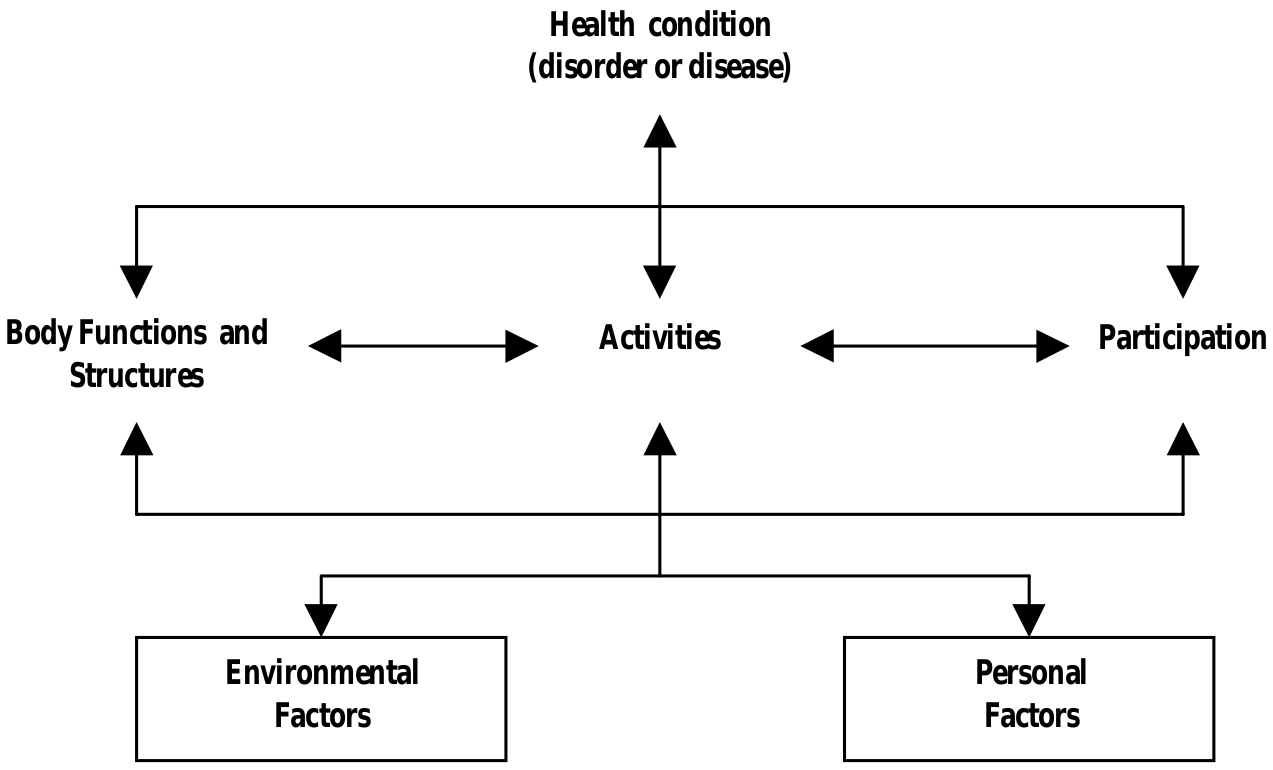
\includegraphics[width=0.65\textwidth]{icf_interaction.png}
\caption{Interactions between the components of~\ac{icf}.}
\label{fig:icf_interaction}
\end{figure}

Researchers have developed and improved several techniques to model users for 
the past 20 years~\citep{petrelli_user_centered_1999} \citep{fink_adaptable_1997}. 
Modelling users needs to gather knowledge about their capabilities, drawbacks and 
limitations. During these first decades there was not any official and medical-based 
study to consult about user capabilities. Nevertheless, in 2001 this situation 
changed. Under the \ac{who} coordination the World Health Assembly published the
\ac{icf} document. This document classifies every function state associated with 
health (e.g., diseases, disruptions, injuries and traumas). Its purpose is to 
identify the low-level capabilities relevant to product design in several 
domains. As was written by experts in the area, the \ac{icf} document is a 
reference for identifying several user capabilities in any interaction process. 
This document is organized into two main groups: the one-level and the two-level 
capabilities classification. From the first group the World Health Assembly 
identified the following categories:

\begin{itemize}
  \item Body functions.
  \item Body structures.
  \item Activities and participation.
  \item Environmental factors.
\end{itemize}

Due to the nature of user capabilities, in this dissertation we take the very 
first category as the official reference to model users as it is directly 
related to \ac{hci}. This category encompasses the following functions:

\begin{itemize}
  \item Mental functions.
  \item Sensory functions and pain.
  \item Voice and speech functions.
  \item Neuromusculoskeletal and movement-related functions.
\end{itemize}


\citeauthor{persad_cognitive_2007} also reviewed functional classifications 
and experimental studies to identify the most relevant low-level skills for 
designing products within the cognitive, motor and sensory domain:

\paragraph*{Sensory capabilities}
\subparagraph*{Visual capabilities} Several sensory capabilities are known to 
deteriorate with ageing~\citep{persad_exploring_2006}. Thus, 
\citeauthor{persad_exploring_2006} stated that the following functions seem to 
account for most of visual disability:

\begin{itemize}
  \item Visual acuity.
  \item Contrast sensitivity.
  \item Colour perception.
  \item Useful field of view.
  \item Stereopsis.
\end{itemize}


\subparagraph*{Hearing capabilities} Loss of hearing capabilities may directly 
affect the speech interaction with the device. The main low-level hearing 
functions to guarantee the interaction are the following:

\begin{itemize}
  \item Pure tone detection thresholds.
  \item Speech detection and recognition discrimination thresholds.
  \item Sound localization.
\end{itemize}

% \subparagraph*{Environmental effects}
% The level of illumination, noise, weather, etc. are several environment features 
% which might affect user capabilities.

\paragraph*{Cognitive capabilities}
The product's user interface must be usable and accessible enough to guarantee 
that users easily understand the interaction. The following capabilities are 
related to the human cognitive domain:

\begin{itemize}
 \item Working memory performance.
 \item Long term memory.
 \item Mental models, planning and problem solving.
 \item Language and communication capabilities.
\end{itemize}

\paragraph*{Motor capabilities}
\subparagraph*{Upper limb capabilities}
There are many conditions that affect manipulating a product (e.g., arthritis, 
stroke, multiple sclerosis, head injury, cerebral palsy and missing or damaged 
limbs). These problems directly reduce grasp forces, range of motion and fatigue 
thresholds~\cite{persad_characterising_2007}.

The following areas are highlighted within motor capabilities:
\begin{itemize}
  \item Reach ranges for each arm.
  \item Grasping, dexterity and force exertion.
  \item Two handed actions and coordination.
\end{itemize}

\subparagraph*{Gross body movement capabilities}
Usually products require certain user mobility degree. 
\\
Besides, \citeauthor{persad_characterising_2007} provide six general categories 
for product features and their interface classification. For this classification 
their toaster case study is considered (see Table~\ref{tbl:persad_product_interface}).

\begin{table}
  \caption{Product interface classification by~\citet{persad_characterising_2007}.}
  \label{tbl:persad_product_interface}
\footnotesize
\centering
    \begin{tabular}{l l}
    \hline
    \textbf{Feature type} & \textbf{Examples} \\
    \hline
    Product chassis & Handles, gripping surface \\
    Displays and indicators & Visual and auditory displays \\
    Controls and control groups & Discrete controls (Button, Switch) and continuous\\
    & controls (Slider, Knob, thumb, wheel, dial, joystick). \\
    & Control groups \textit{Keypad} \\
    Material/media input and output & Slots (toaster slots), powered and un-powered\\
    & bays and trays, doors, lids and covers\\
    Connectors for energy and data & Power and data connectors \\
    Software interfaces & Navigation menus and GUI objects \\
    \hline
  \end{tabular}
\end{table}